\section{Interferometry and the Inverse Problem}\label{intro}
Radio Antennas in Astronomy require a sub-arcsecond angular resolution. For a single dish antenna, the angular resolution is $ \theta \approx \lambda / D$ radians, which leads to impossibly large diameters for radio wavelengths. Interferometers, where several dishes act as a single instrument, can achieve a high angular resolution for an economical price.  (Radio Astronomy has a lot of interest in Interferometers, building VLA, ALMA, LOFAR and planning SKA). However Interferometers do not observe the sky directly. Each antenna pair measures a Fourier component of the observed image. Furthermore the Fourier space is not fully samnpled, it is incomplete. The task is to reconstruct an image in Pixel space from an incomplete set of Fourier measurements (Visibilities). From here on forward term Visibility is used. It is interchangeable with Fourier Component.

Each antenna pair, quadratic number of data points with the number of antennas: a lot of data)(An interferometer does not observe the image directly. Simplified, each antenna pair observes a Fourier component of the An Antenna Pair measures a fourier component of the image.) (If all the fourier components are measured, the observed image could be retrieved by calculating the inverse fourier transform. However, only a limited set of visibilites can be measured.)(Inverting the problem results in an image with artefacts (Dirty Image).) (Clean can solve it for the current class of interferometers)

(Future Interferometers like the Square Kilometer Array do introduce additional problems in the inverse Problem.)(Modelling the new effects)(while being able to handle the large amount of data.)

% The Inverse Problem. Radio Astronomy has come up with the CLEAN class Algorithms\cite{hogbom1974aperture} \cite{schwab1984relaxing} \cite{rich2008multi}\cite{rau2011multi} that work well in practice for current radio interferometers.
%The theory of Compressed Sensing \cite{candes2006robust} \cite{donoho2006compressed}


\subsection{Simplified Inverse Problem}
For the current class of interferometers, retrieving the observed image of the sky is calculating the Inverse Fourier Transform of the measured Visibilities. (This is a simplification of the actual problem, which does not hold true for future instruments like SKA. How the Inverse Problem changes for future instruments is handled in section \ref{radio}). Since the Visibility Space is undersampled, the resulting image is 'dirty', as it contains effects from the instrument. The effects of the instrument can be modelled as a Point Spread Function (PSF). The Dirty Image is the Result of the True Image convolved with the PSF, $D_{True} \star PSF = D_{Dirty}$. Figure \ref{intro:inverse_problem} shows an example of the PSF, Dirty Image and True Image.  Since only the PSF and the Dirty Image are known, one tries to deconvolve the Dirty Image and retrieve the True Image.
\begin{figure}[h!]
	\centering
	\begin{subfigure}[b]{0.3\linewidth}
		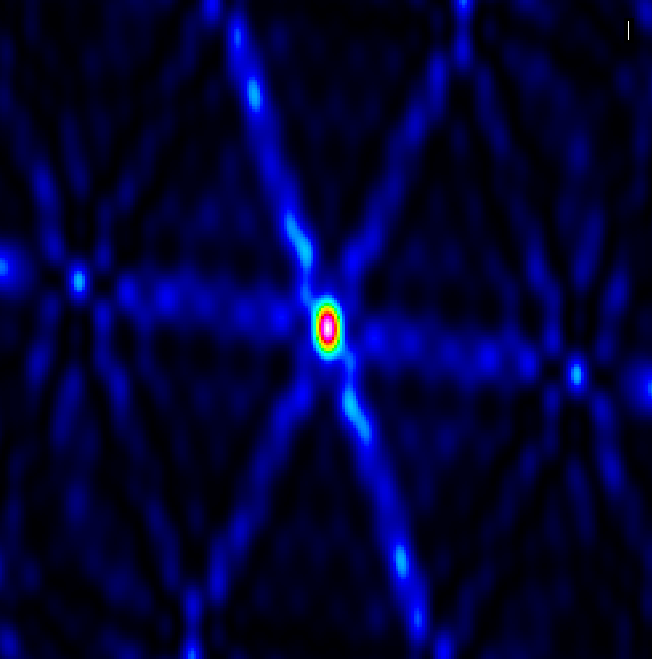
\includegraphics[width=\linewidth]{./chapters/01.intro/img/PSF.png}
		\caption{Point Spread Function (PSF)}
	\end{subfigure}
	\begin{subfigure}[b]{0.3\linewidth}
		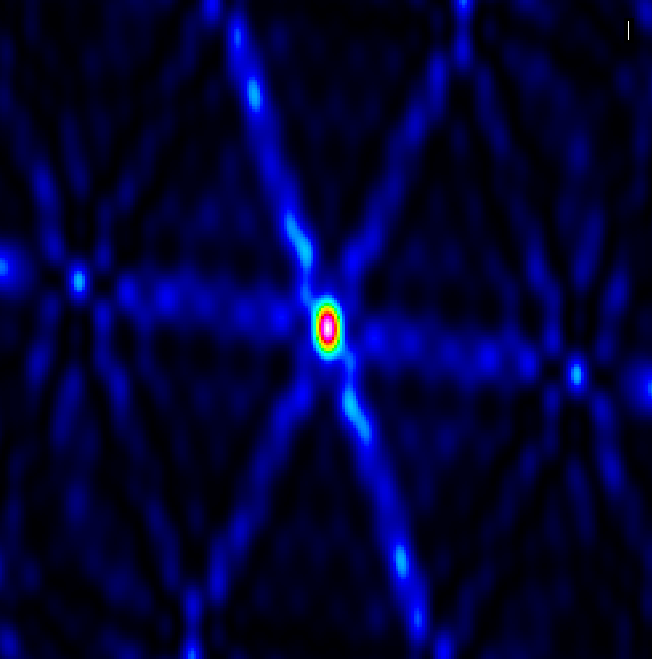
\includegraphics[width=\linewidth]{./chapters/01.intro/img/PSF.png}
		\caption{Dirty Image}
	\end{subfigure}
	\begin{subfigure}[b]{0.3\linewidth}
		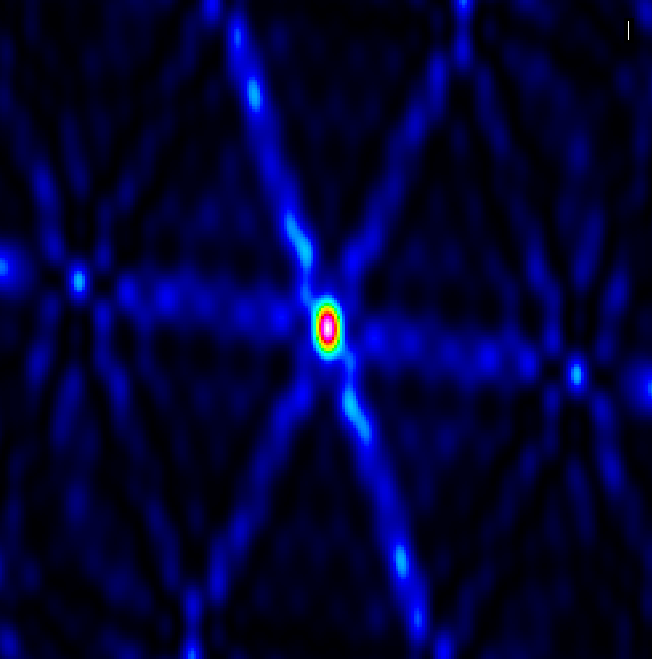
\includegraphics[width=\linewidth]{./chapters/01.intro/img/PSF.png}
		\caption{True Image}
	\end{subfigure}
	\caption{The Inverse Problem: Finding the true image of the sky when only the PSF and the observed image are known.}
	\label{intro:inverse_problem}
\end{figure}

The Dirty Image is the result of the Inverse Fourier Transform, the PSF on the other hand follows directly from the antenna configuration. Figure \ref{intro:ANT_UV_PSF} shows an example of the VLA instrument. 

\begin{figure}[h!]
	\centering
	\begin{subfigure}[b]{0.3\linewidth}
		 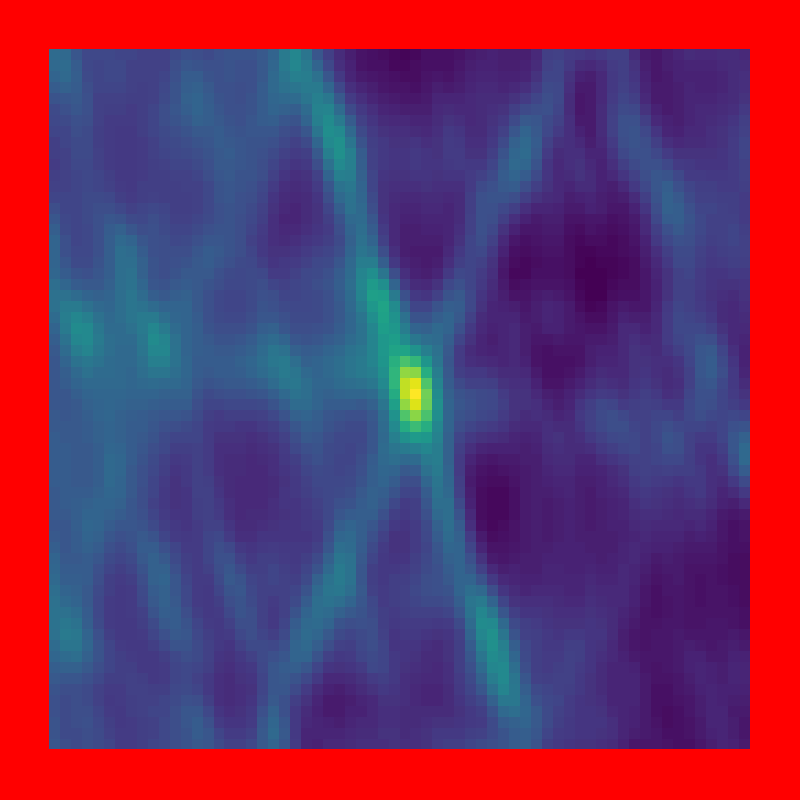
\includegraphics[width=\linewidth, trim={16px 16px 16px 16px}, clip]{./chapters/01.intro/img/mytest.png}
		 \caption{Antenna Configuration}
	\end{subfigure}
	\begin{subfigure}[b]{0.3\linewidth}
		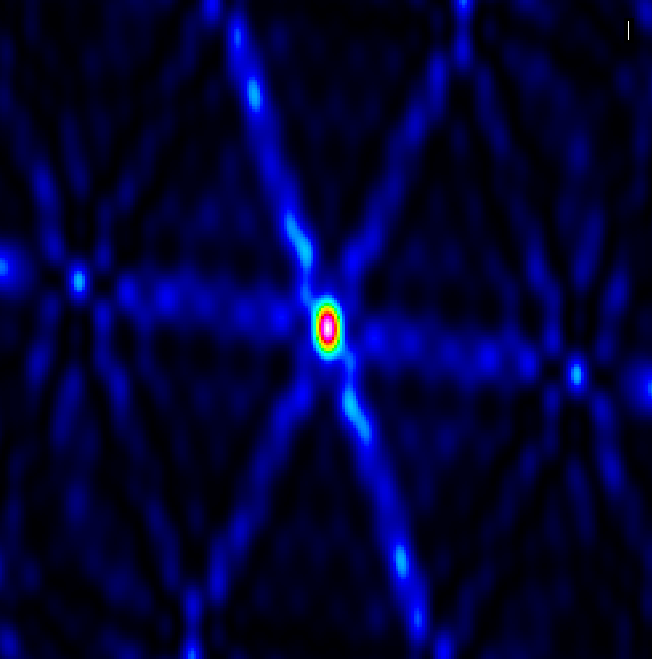
\includegraphics[width=\linewidth]{./chapters/01.intro/img/PSF.png}
		\caption{UV Space}
	\end{subfigure}
	\begin{subfigure}[b]{0.3\linewidth}
	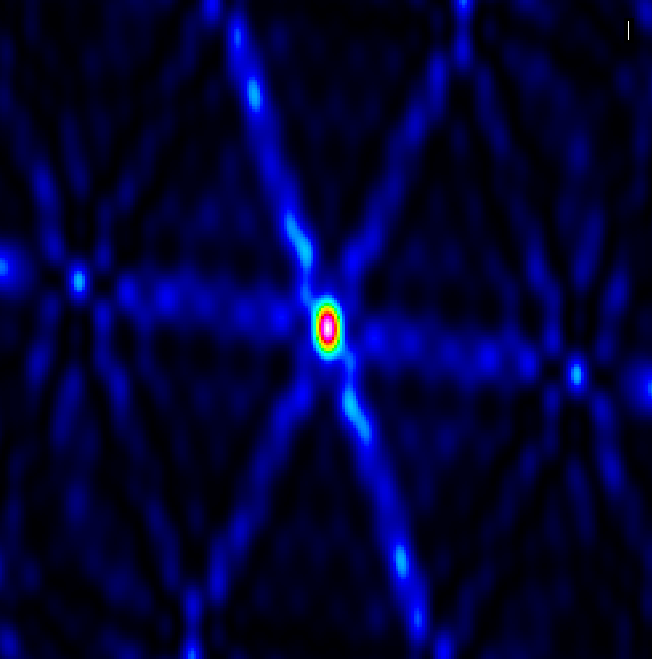
\includegraphics[width=\linewidth]{./chapters/01.intro/img/PSF.png}
	\caption{Point Spread Function (PSF)}
	\end{subfigure}
	\caption{The Antenna Configuration sets up the UV Space. The UV Space dictates the PSF.}
	\label{intro:ANT_UV_PSF}
\end{figure}

Each antenna pair samples a point in the UV Space. The distance between the antenna pair is called the baseline. Shorter baselines sample UV-Points closer to the center, while longer baselines sample points further away.  Each point in the UV Space represents a frequency Visibilities of the observed image: High frequency components are located away from the center and low frequency components are towards the center. Since each antenna pair contributes a Visibility, an Interferometer of $N$ antennas measures $(N-1)/2$ Visibilities. The configuration of the antenna sets up which points are sampled in the UV Space. 


\subsection{Deconvolution with CLEAN}
Clean follows from the simplified Inverse problem. The dirty image results from the True image getting convolved with the PSF. It searches to deconvolve the dirty image with the PSF and retrieve the actual sky image.

\begin{figure}[h!]
	\centering
	\begin{subfigure}[b]{0.4\linewidth}
		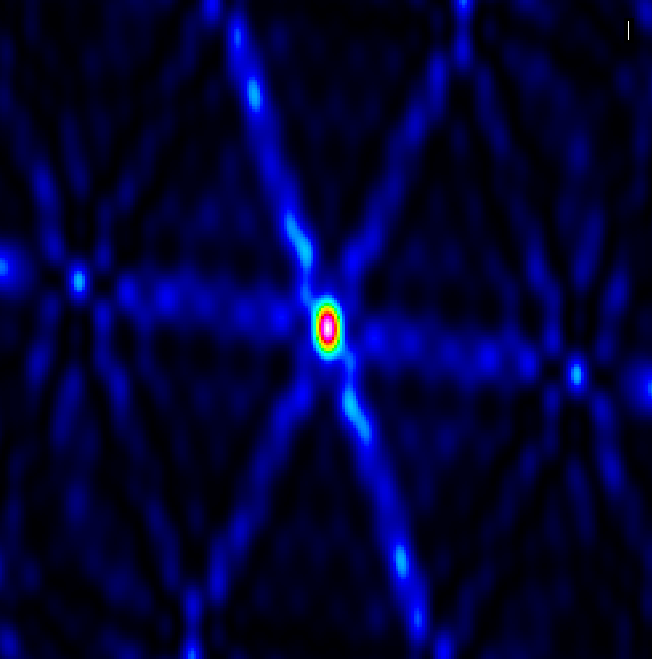
\includegraphics[width=\linewidth]{./chapters/01.intro/img/PSF.png}
		\caption{Dirty Image}
	\end{subfigure}
	\begin{subfigure}[b]{0.4\linewidth}
		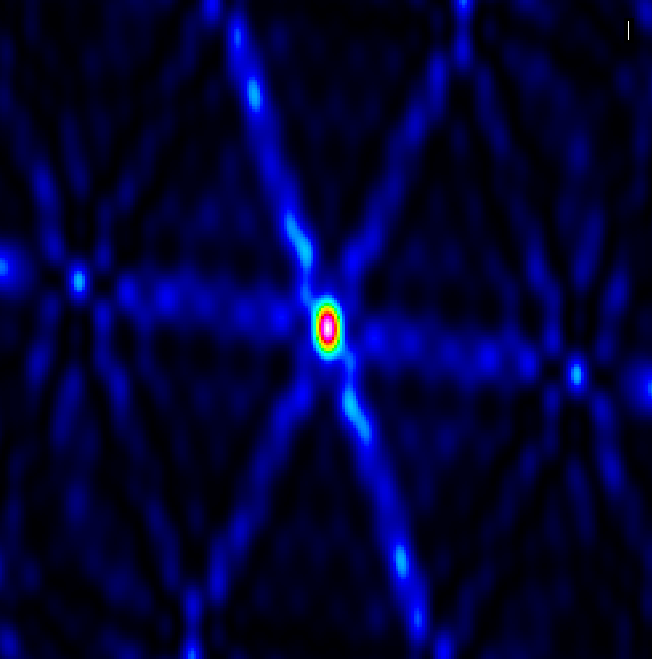
\includegraphics[width=\linewidth]{./chapters/01.intro/img/PSF.png}
		\caption{True image of the sky.}
	\end{subfigure}
	\caption{The Inverse Problem: Finding the true image of the sky when only the PSF and the observed image are known.}
	\label{intro:deconvolve}
\end{figure}

Clean implementation, removing the biggest peak. Early stopping


\subsection{Compressed Sensing for Interferometry}

\begin{equation}\label{intro:deconvolution}
I \star PSF = I_Dirty
\end{equation}

(Clean Approximates the solution)(Theoretical guarantees)

clean in CS formulation. Prior knowledge of the sky. Theory of compressed sensing states that we can retrieve the true image potentially below the Nyquist Shannon Rate.

Another way of looking at the inverse problem is to formulate it as the solution to an underdetermined system. \eqref{intro:underdetermined}. In our case, $y$ are the observed Fourier components, $x$ is the reconstructed image and $F$ is the Fourier Transform. We try to find $x$ that explain the observations $y$, but since it is an under determined system, there are multiple solutions. The intuitive way to solve it is to increase the number of observations until we have a fully-determined system. However, this is not necessary. With the theory of Compressive Sensing one can find the correct solution by exploiting the fact that $x$ is compressible.

It turns out that many natural signals are compressible. A picture taken by an ordinary camera produces megabytes of data, but after compression only a fraction of the original need to stored. JPEG2000 uses the Wavelet Transform and only needs to store a limited number of Wavelet coefficients. More formally, if $W$ is the Wavelet transform and $e$ a natural Image, $We = \alpha$. $\alpha$ are the wavelet coefficients. Since natural images are compressible in the wavelet domain, $\alpha$ is sparse (contains mostly zeroes) and can be stored using less space than the image $e$.

Coming back to the original underdetermined system \eqref{intro:underdetermined}, we introduce a Dictionary $D$ which contains our basis functions. We assume that $x$ is compressible using the Dictionary: $D\alpha = x$ and $\alpha$ has only a few non-zero entries. Instead of solving \eqref{intro:underdetermined} directly, we substitute $x$ with $D\alpha$ and search for the solution that has the fewest non-zero elements in $\alpha$. We arrive at the minimization problem \eqref{intro:ssparseland}, where $\mathit{ind}()$ is the indicator function. 

S- Compressible. Under what circumstance is $D\tilde{\alpha} = x$. In compressed Sensing states that if we have a "good" dictionary, i.e. one where $x$. Also there are few limitations on $D$. It can be the Wavelet transform, Fourier Transform, or even a combination of the two.

\begin{equation}\label{intro:ssparseland}
\tilde{\alpha} =  \underset{\alpha}{arg min} \: \mathit{ind}(D\alpha) \quad s. t. \quad FD\alpha = y
\end{equation}

Non-convex optimization, real environment has noise. It can be shown that the L1 norm approximates the indicator function.

\begin{equation}\label{intro:sparseland}
\begin{split}
x  =  D_{\alpha}
\end{split}
\quad , \quad
\begin{split}
x &\in \mathcal{R}^n\\
\alpha &\in \mathcal{R}^k\\
D &\in \mathcal{R}^{n \times k}
\end{split}
\quad with \quad
\begin{split}
n \ll k
\end{split}
\end{equation}

Plausible Image, sparsity

\begin{equation}\label{cs:noiseless}
\tilde{\alpha} =  \underset{\alpha}{arg\: min}
\end{equation}

